\chapter{Hardware design}

\section{Encoder}

\subsection{Højpasfilter}

\subsection{Zero Crossing Detector}

\newpage

\section{Decoder}

\subsection{Båndpasfilter}
\begin{figure}[htbp]
	\centering
	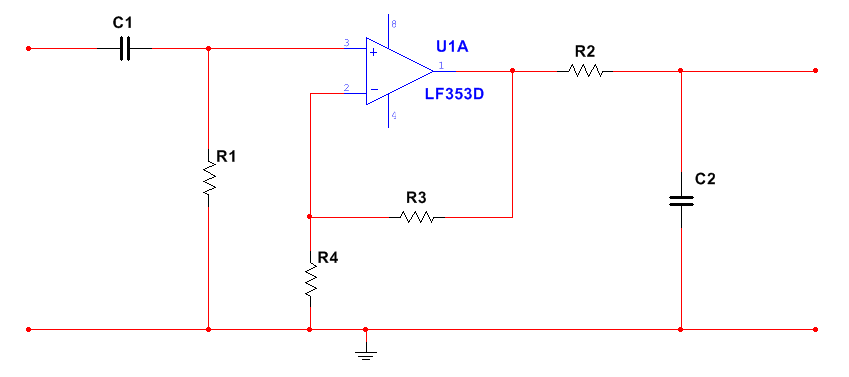
\includegraphics[width=0.70\textwidth]{billeder/HWdesign/BAANDPAS_UV.png}
	\caption{Båndpas uden værdier}
	\label{fig:BAANDPAS_UV}
\end{figure}

Båndpasfilteret har til opgave at filtrere alle signaler med frekvenser over og under 120 kHZ fra samtidig med at det forstærker signalet i båndpasset. Forstærkningen opnås ved at koble en ikke inverterende OpAmp med modstande, hvis størrelse afhænger af den ønskede forstærkning, mellem et højpasfilter og lavpasfilter som illustreret på figur \ref{fig:BAANDPAS_UV}.

Da vi ønsker at forstærke 120 kHz signalet, designes højpasfilteret således at knækfrekvensen udregnes til 110 kHz, og for lavpasfilteret beregnes en knækfrekvens på 130 kHz. 

\begin{align}
R = \frac{1}{2 \cdot \pi \cdot f_c \cdot C } 
\end{align}

Fælles for begge filtre vælges en kondensator med en værdi på 1,0 nF. Med denne værdig kan de to modstande i henholdsvis lavpas- og højpasfilteret beregnes.

Højpasfilterets modstand:
\begin{align}
R_1 = \frac{1}{2 \cdot \pi \cdot 130000 \cdot 1,0 \cdot 10^{-9}} = 1447 \Omega
\rightarrow R_1 > 1447 \Omega
\end{align}
$R_1$ vælges da til 1,6 k$\Omega$


Lavpasfilterets modstand:
\begin{align}
R_2 = \frac{1}{2 \cdot \pi \cdot \ 110000 \cdot 1,0 \cdot 10^{-9}} = 1225 \Omega
\rightarrow R_2 < 1224 \Omega
\end{align}
$R_2$ vælges da til 1,1 k$\Omega$

Da det ikke kan undgås at 120 kHz signalet bliver dæmpet både gennem højpasfilteret og lavpasfilteret er det nødvendigt at forstærke signalet ved hjælp af en LF353 OpAmp.
Ligningen for udregning af udgangsspændingen er som følgende:
\begin{align}
V_{out} = (1 + \frac{R_3}{R_4}) \cdot V_{in}
\end{align} 

Ved at vælge $R_4$ til 10 k$\Omega$ kan forstærkningen nemt reguleres med $R_3$.
Ved målinger på indgangssignalet før operationsforstærkeren kan vi fastslå indgangsamplituden til at være 8,0 V. Da udgangssignalet ledes gennem en diode der fjerner de negative halvperioder vil amplituden blive halveret gennem denne. Samtidig er der dæmpning i lavpasfilteret og der vil derfor være brug for en mere end en fordobling i forstærkeren. 

\begin{align}
R_4 = (\beta - 1) \cdot R_3 = (3 - 1) \cdot 10000 = 20000 \Omega
\end{align} 
$R_4$ er valgt til 20000 $\Omega$ så signalet derved bliver forstærket 3 gange.

Der er som nævnt valgt en LF353 OpAmp. Denne er valgt ud fra at den har en bred båndbredte, en hurtig sætte tid og lav støj på indgangene. 

Med alle de beregnede komponentværdier kan det endelige schematic designes. Det endelige design er vist på figur \ref{fig:BAANDPAS_MV} 

\begin{figure}[htbp]
	\centering
	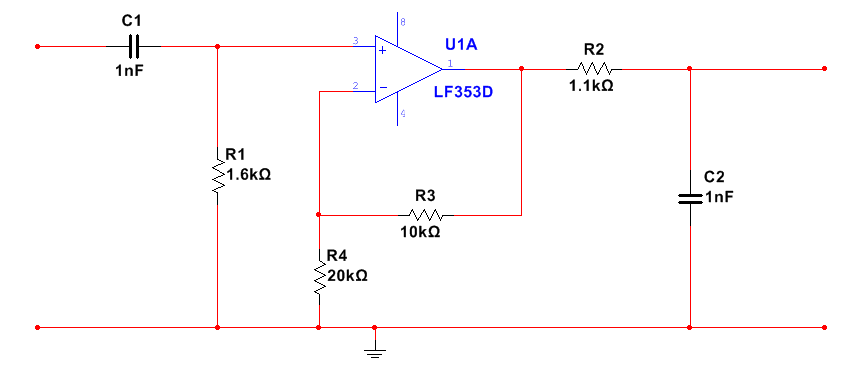
\includegraphics[width=0.70\textwidth]{billeder/HWdesign/BAANDPAS_MV.png}
	\caption{Båndpas uden værdier}
	\label{fig:BAANDPAS_MV}
\end{figure}
 

\newpage

\subsection{Envelope Detector}
